\section{Signed square cycles: the verified predecessor}
\label{sec:graphs}

\subsection{The optimization problem}

For \(n\ge5\), let \(C_n(1,2)\) have vertex set \(\Z/n\Z\), with an
undirected edge between vertices at cyclic distance one or two. Assign
each edge an independent sign \(+1\) or \(-1\). The signed adjacency matrix
\(A\) is real and symmetric, and
\[
\rho(A)=\max_{\lambda\in\operatorname{spec}(A)}|\lambda|=\|A\|.
\]
The question is to minimize this number over all signs.

Write \(a_i\) for the sign of \(\{i,i+1\}\), and \(b_i\) for that of
\(\{i,i+2\}\). Switching signs at vertices conjugates \(A\) by a diagonal
matrix with entries \(\pm1\), preserving its spectrum. The invariants
\[
\tau_i=a_i a_{i+1}b_i,\qquad \alpha=\prod_i a_i
\]
are the triangle signs and the Hamilton-cycle sign product. They determine
a labeled switching class: switch to \(a_0=\cdots=a_{n-2}=1\),
\(a_{n-1}=\alpha\), and recover \(b_i=\tau_i a_i a_{i+1}\).
There are \(2^{n+1}\) such classes. Counts of minimizing switching classes
below are not counts of individual raw edge assignments.

Suvagiya's Conjecture 28 proposed a constant optimum for \(n=8m\ge32\)
\cite{Suvagiya}. A prior public counterexample at \(32\) vertices already
refuted that assertion, but explicitly left the exact optimum open
\cite{Trure}. The incoming report supplied the stronger complete answer
\cite{IncomingCycle}.

\begin{theorem}[Incoming result, independently revalidated]
\label{th:priorcycle}
Let
\[
F(u)=\sqrt{4+\sqrt{8+u+\sqrt{26-3u}}},\qquad
P=(+,+,-,+,-,-,+,-).
\]
For every \(m\ge4\), the minimum for \(C_{8m}(1,2)\) is
\[
F(2\cos(\pi/m)).
\]
Its eight labeled minimizing switching classes have triangle signs given
by the rotations of \(P^m\), and \(\alpha=-1\).
The next distinct radius is \(F(2)\); all other classes have
radius at least \(1397/500=2.794\).
\end{theorem}

\subsection{Why the finite certificate proves an infinite family}

For a word \(w=(t_0,\ldots,t_{k-1})\), let \(H(w)\) be the signed square of
a path on \(k+2\) vertices, with all distance-one signs positive and
distance-two signs \(t_i\). To test \(\|H(w)\|<T\), test positive
definiteness of both \(TI-H(w)\) and \(TI+H(w)\).

After eliminating all but the last two vertices in \(TI-H(w)\), write the
remaining Schur block as
\(\left(\begin{smallmatrix}a&b\\b&c\end{smallmatrix}\right)\).
Appending a sign \(t\) gives
\begin{equation}
(a,b,c)\longmapsto
\left(c-\frac{b^2}{a},\ -1+\frac{bt}{a},\ T-\frac1a\right).
\label{eq:schur}
\end{equation}
The updated block is positive definite precisely when \(a'>0\) and
\(a'c'>(b')^2\). The initial block is \((T,-1,T)\). Alternating vertex
switches turn the second shifted matrix into the same calculation with
all \(t_i\) negated.

At \(T=1397/500\), exact enumeration at length \(27\) retains exactly the
eight windows of the periodic word \(P\). The overlapping prefixes have
unique continuations. Any signed cycle with \(n\ge31\) and norm below \(T\)
must therefore have this period-eight triangle word. This follows because
the norm of an induced path compression cannot exceed the whole matrix norm.

For that periodic family, diagonalize translation by eight. The boundary
phase satisfies \(z^m=\alpha\). With \(u=z+z^{-1}\) and \(h=x^2-4\), the
characteristic polynomial of an eight-dimensional block is
\[
h^4-(16+2u)h^2+u^2+19u+38.
\]
Its norm is \(F(u)\). Since \(F\) is strictly increasing on \([-2,2]\),
the largest allowed \(u\) is \(2\) for positive holonomy, and
\(2\cos(\pi/m)\) for negative holonomy. Both resulting radii are below
\(T\), proving the optimum and equality statement.

The predecessor's rational Schur calculation, dense integer determinant
calculation, and independent signed-permutation determinant calculation
were all replayed successfully. Its four small-cycle checks were also
replayed. This is a complete proof with a finite exact computation; it is
not a Lean formalization of the graph result.

\clearpage
\section{Seven new graph cases, including the fifty-vertex optimum}
\label{sec:newgraphs}

\subsection{A complete certificate for six further sizes}

\begin{theorem}[Six new alternating optima]
\label{th:six}
For
\[
n\in\{34,36,38,42,44,46\},
\]
the unrestricted minimum is
\begin{equation}
G(n)=2\sqrt{\cos^2(\pi/n)+\cos^2(2\pi/n)}.
\label{eq:alternating}
\end{equation}
Exactly two labeled switching classes minimize it: alternating triangle
signs, with Hamilton-cycle sign product \(\alpha=-1\).
\end{theorem}

\begin{proof}
For each \(n\), choose the rational threshold \(T\) in the table below.
The exact recursion \eqref{eq:schur} lists every word of length \(n-4\)
whose path norm is below \(T\). Complete each such word in every one of
the \(2^4\) ways, and retain a cycle word only when every cyclic window
of length \(n-4\) is on the passing list. In each case the sole surviving
rotation class is alternating.

This necessary condition is complete as an exclusion argument. A window
occupies \(n-2\) consecutive vertices; the two omitted consecutive vertices
leave its endpoints at cyclic distance three, so there is no extra seam
edge in the induced graph. Any whole-cycle norm \(<T\) passes every
compression test. After reduction to rotation representatives, test both
values of \(\alpha\) by exact integer elimination on
\((\operatorname{den}T)(TI\pm A)\). Only \(\alpha=-1\) passes.

\begin{center}
\begin{tabular}{rrrrr}
\toprule
\(n\)&\(T\)&window length&passing path words&cyclic rotation classes\\
\midrule
34&\(281/100\)&30&98&1\\
36&\(281/100\)&32&108&1\\
38&\(281/100\)&34&92&1\\
42&\(281/100\)&38&70&1\\
44&\(703/250\)&40&394&1\\
46&\(703/250\)&42&422&1\\
\bottomrule
\end{tabular}
\end{center}

These are exhaustive exact computations in
\code{checks/graphs/verify_even_extensions.py}, with every prefix count
recorded in its JSON certificate. Bareiss elimination computes leading
principal minors without row swaps; their positivity is Sylvester's
criterion. No floating-point comparison is used.

For completeness, the alternating family has two-dimensional Fourier
blocks
\[
\begin{pmatrix}
2\cos(2\theta)&2\cos\theta\\
2\cos\theta&-2\cos(2\theta)
\end{pmatrix},
\qquad \theta=(2j+1)\pi/n
\]
at negative holonomy. The squared block norm is
\(4(\cos^2\theta+\cos^2 2\theta)\).
Putting \(x=\cos^2\theta\) makes the expression divided by four
\(4x^2-3x+1\), a convex polynomial. For even \(n\ge8\) its maximum on
the allowed values is at \(x=\cos^2(\pi/n)\): at the opposite extreme
the allowed value is \(0\) or \(\sin^2(\pi/n)\). If it is \(0\),
\(x_{\max}>3/4\) implies \(4x_{\max}^2-3x_{\max}+1>1\).
If it is \(1-x_{\max}\), subtracting the two polynomial values gives
\(2x_{\max}-1>0\).
This proves \eqref{eq:alternating}.
The positive-holonomy radius is \(2\sqrt2>T\).

Finally, \(G(n)<T\) is certified using a rational lower bound for \(\pi\)
from Machin's identity and the alternating arctangent series, followed
by \(\cos x\le1-x^2/2+x^4/24\). Hence the candidate exists below the
threshold that excludes all competitors. The two phases of alternation
give exactly two labeled switching classes.
\end{proof}

\subsection{A new exact optimum at fifty vertices}
The preceding incoming report leaves exact optima at large lengths not
divisible by eight undetermined. The following theorem settles its first
new case investigated here at which the alternating family fails. This is
a new result relative to the 46 inspected incoming archives; no worldwide
priority claim is made.

Write $a_i\in\{\pm1\}$ for the sign on the edge $\{i,i+1\}$ and
$b_i\in\{\pm1\}$ for the sign on $\{i,i+2\}$, with indices modulo $50$.
The triangle signs and Hamilton-cycle holonomy are
\[
 \tau_i=a_i a_{i+1}b_i,\qquad \alpha=\prod_{i=0}^{49}a_i.
\]
Vertex switching preserves these data, and they determine a labeled
switching class: switch to $a_0=\cdots=a_{48}=1$, $a_{49}=\alpha$,
then recover $b_i=\tau_i a_i a_{i+1}$.

\begin{theorem}[The fifty-vertex optimum]
Let $\rho_{50}$ be the minimum spectral radius over all independent edge
signings of $C_{50}(1,2)$. Put
\[
 B=(-,-,+,-,+,+,-,+),\qquad W=B^6(-,+).
\]
Precisely the switching classes with $\alpha=+1$ and triangle word a
cyclic rotation of $W$ or $-W$ minimize the spectral radius. These are
$100$ distinct labeled switching classes. Moreover,
\[
  \boxed{2.811568906156<\rho_{50}<2.811568906157.}
\]
An exact algebraic specification is
$\rho_{50}=\sqrt{y_{\max}}$, where $y_{\max}$ is the largest real root
of the degree-$25$ polynomial $Q$ recorded in the coefficient table below.
Every other switching class has spectral radius at least
$7029/2500=2.8116$.
\end{theorem}

\begin{proof}
Set $T=7029/2500$. For a triangle word $w$ of length $k$, let $H(w)$
be the $(k+2)$-vertex path with all length-one signs positive and
length-two signs given by $w$. Retain a word exactly when both
$TI-H(w)$ and $TI+H(w)$ are positive definite. Starting from the empty
word and extending only retained prefixes exhausts all passing words,
because each shorter path is a principal submatrix.

The exact Schur update on the last two vertices is
\[
 (a,b,c)\longmapsto
 \left(c-\frac{b^2}{a},\,-1+\frac{bt}{a},\,T-\frac1a\right),
\]
for appended sign $t$. Start with $(T,-1,T)$; the second shifted matrix
uses $-t$. The updated block passes precisely when $a'>0$ and
$a'c'>(b')^2$ in both cases. All calculations use rational arithmetic.
At triangle length $46$ there are $324$ passing words. Append all four
remaining signs to each of them and retain a length-$50$ word only if
all its cyclic length-$46$ windows pass. There are exactly two resulting
rotation classes, represented by $W$ and $-W$.

The exhaustive local path classification is checked by two independent
algorithms in the package. The first uses the Schur recurrence; the
second constructs determinants by summing signed permutation products,
using only integer arithmetic and the band width of the actual path
matrices. They agree on every prefix count and every surviving word.
The cyclic completion and full-matrix tests are exact finite calculations
in the first verifier. The complete lists and checks are supplied as
executable certificates.

Any consecutive $48$ vertices in $C_{50}(1,2)$ induce such a path:
the two endpoints have cyclic distance three, so no extra edge joins
them. Its matrix norm is bounded by the whole symmetric-matrix norm.
Consequently every signing with radius $<T$ must have one of these two
triangle words, up to rotation. There remain just two holonomies for
each word. Exact fraction-free elimination of the full matrices
$7029I\pm2500A$ shows that $\alpha=+1$ passes both Sylvester tests,
whereas $\alpha=-1$ fails. The first $49$ leading minors are positive
in each failed test, and the final determinant is negative. Thus no
additional signing can have radius $<T$.

Negating every edge changes every triangle sign to its negative and,
because $50$ is even, preserves $\alpha$. It takes $A$ to $-A$, so the
two surviving rotation classes have equal spectral radius. Both are
therefore global minimizers. Each word has primitive period $50$ and
their rotation orbits are disjoint, giving exactly $100$ labeled
switching classes.

The characteristic polynomial of either minimizing representative is
$\det(xI-A)=Q(x^2)$. The supplied checker computes it from integer traces
$\operatorname{tr}(A^j)$ by Newton's identities. For
$r_-=2811568906156/10^{12}$ and
$r_+=2811568906157/10^{12}$, exact leading-minor sign counts show
that $r_-I-A$ and $r_-I+A$ each have exactly one negative eigenvalue,
while both shifts at $r_+$ have none. This proves the strict interval,
and also shows that the interval contains exactly one positive
eigenvalue. The characteristic polynomial specifies the value exactly.
\end{proof}

The alternating family's best value is
$2\sqrt{\cos^2(\pi/50)+\cos^2(2\pi/50)}>2.814$.
For an exact comparison, use $\pi<22/7$ and
$\cos u\ge1-u^2/2$: setting $v=11/175$, rational arithmetic gives
\[
 4\left((1-v^2/2)^2+(1-2v^2)^2\right)>(2814/1000)^2.
\]
Thus the improvement over alternation is strict and does not rely on
numerical eigenvalue estimates.

\paragraph{Polynomial coefficients.}
Write $Q(y)=\sum_{j=0}^{25}q_jy^j$. Its coefficients are
\begin{center}\small
\begin{tabular}{rr@{\qquad}rr}
\hline
$j$&$q_j$&$j$&$q_j$\\\hline
25&1&12&-42556190827574\\
24&-100&11&95424283730427\\
23&4702&10&-173149057931144\\
22&-138186&9&251857479144425\\
21&2846105&8&-290088695299758\\
20&-43660212&7&260508422825773\\
19&517548579&6&-178938476667148\\
18&-4854567112&5&91816438267915\\
17&36601189842&4&-34160308422738\\
16&-224095627758&3&8848896828974\\
15&1121189638159&2&-1499411878484\\
14&-4598060887914&1&148268409185\\
13&15463123646497&0&-6447640168\\\hline
\end{tabular}
\end{center}
No irreducibility assertion is needed. Exact finite enumeration and
the analytic compression argument establish the theorem; this result
has not been formalized in Lean.


\subsection{What the new case reveals}

Together with the revalidated predecessor, Theorem~\ref{th:six} and the
fifty-vertex certificate give exact optima for every even size
\(8\le n\le50\), as well as for every multiple of eight at least \(32\).
At sizes divisible by eight and at least \(32\), the optimal triangle
signs have exact period eight and negative holonomy. At \(50\), the winning
word is six copies of an eight-letter block with an additional two-letter
segment, and its holonomy is positive. One cannot predict the optimizer by
carrying over the best boundary condition from a different cycle length.

\begin{figure}[htbp]
\centering
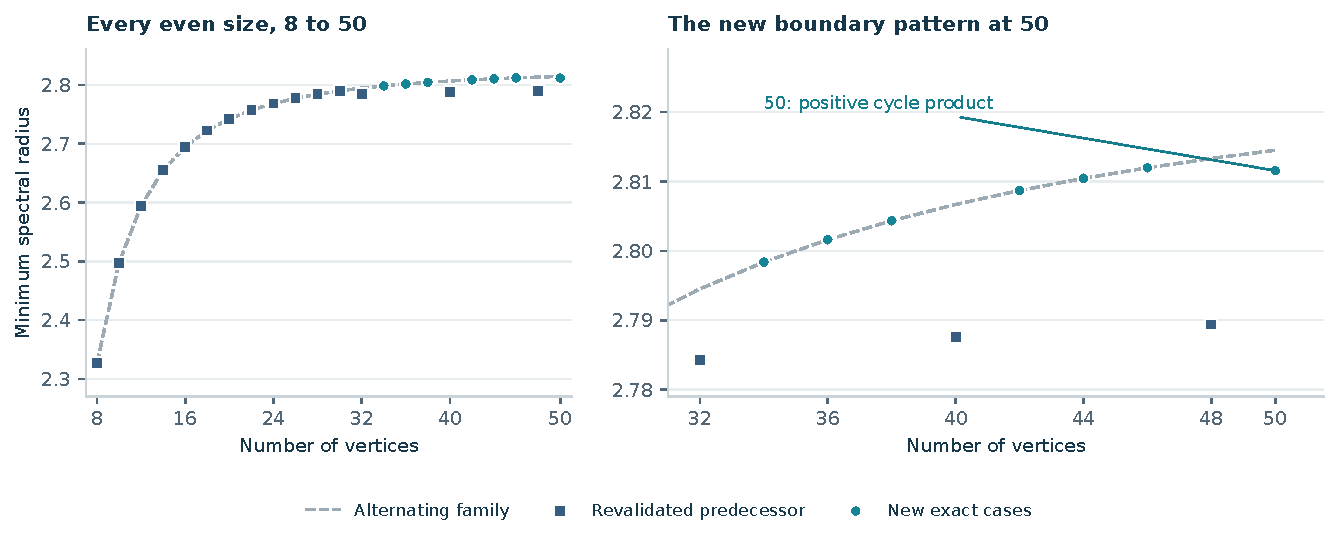
\includegraphics[width=\linewidth]{figures/cycle_optima.pdf}
\caption{Exact minimum formulas or certified values at all even sizes
through fifty. The new cases are highlighted. The thin curve is the
alternating-family value; the points at multiples of eight at least
thirty-two and at fifty fall below it. Decimal plotting is illustrative;
the proof uses exact certificates and formulas.}
\end{figure}

The next focused problem is a uniform description at lengths
\(8m+2\), \(8m+4\), and \(8m+6\). The \(50\)-vertex word is evidence for
a useful defect-pattern search, not a proof that one defect always wins.
The finite-window language can become much larger at a slightly increased
threshold, so there is additional spectral structure to analyze.
